\documentclass[../TDE3.tex]{subfiles}%

\begin{document}
\section[s]"1"{Quelle courbe pour quel circuit~?}
\enonce{%
	\noindent
	\begin{minipage}{0.50\linewidth}
		Um étudiantx distrait, mais surtout maladroitx, rentrant d’une séance de
		travaux pratiques sur l'observation de régimes transitoires sur les circuits
		du premier ordre, fait tomber toutes ses notes qui s’éparpillent. En les
		rangeant, iel retrouve alors 2 courbes expérimentales, tracées en utilisant
		une résistance $R = \SI{1}{k\Omega}$, mais iel ne sait plus à quel montage
		les attribuer.
	\end{minipage}
	\hfill
	\begin{minipage}{0.45\linewidth}
		\begin{center}
			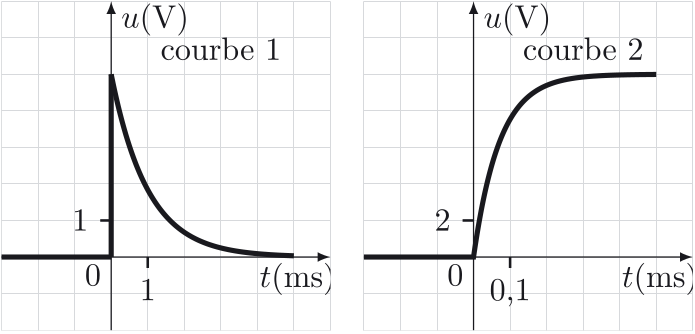
\includegraphics[width=\linewidth]{quellecourbe}
		\end{center}
	\end{minipage}

	\begin{center}
		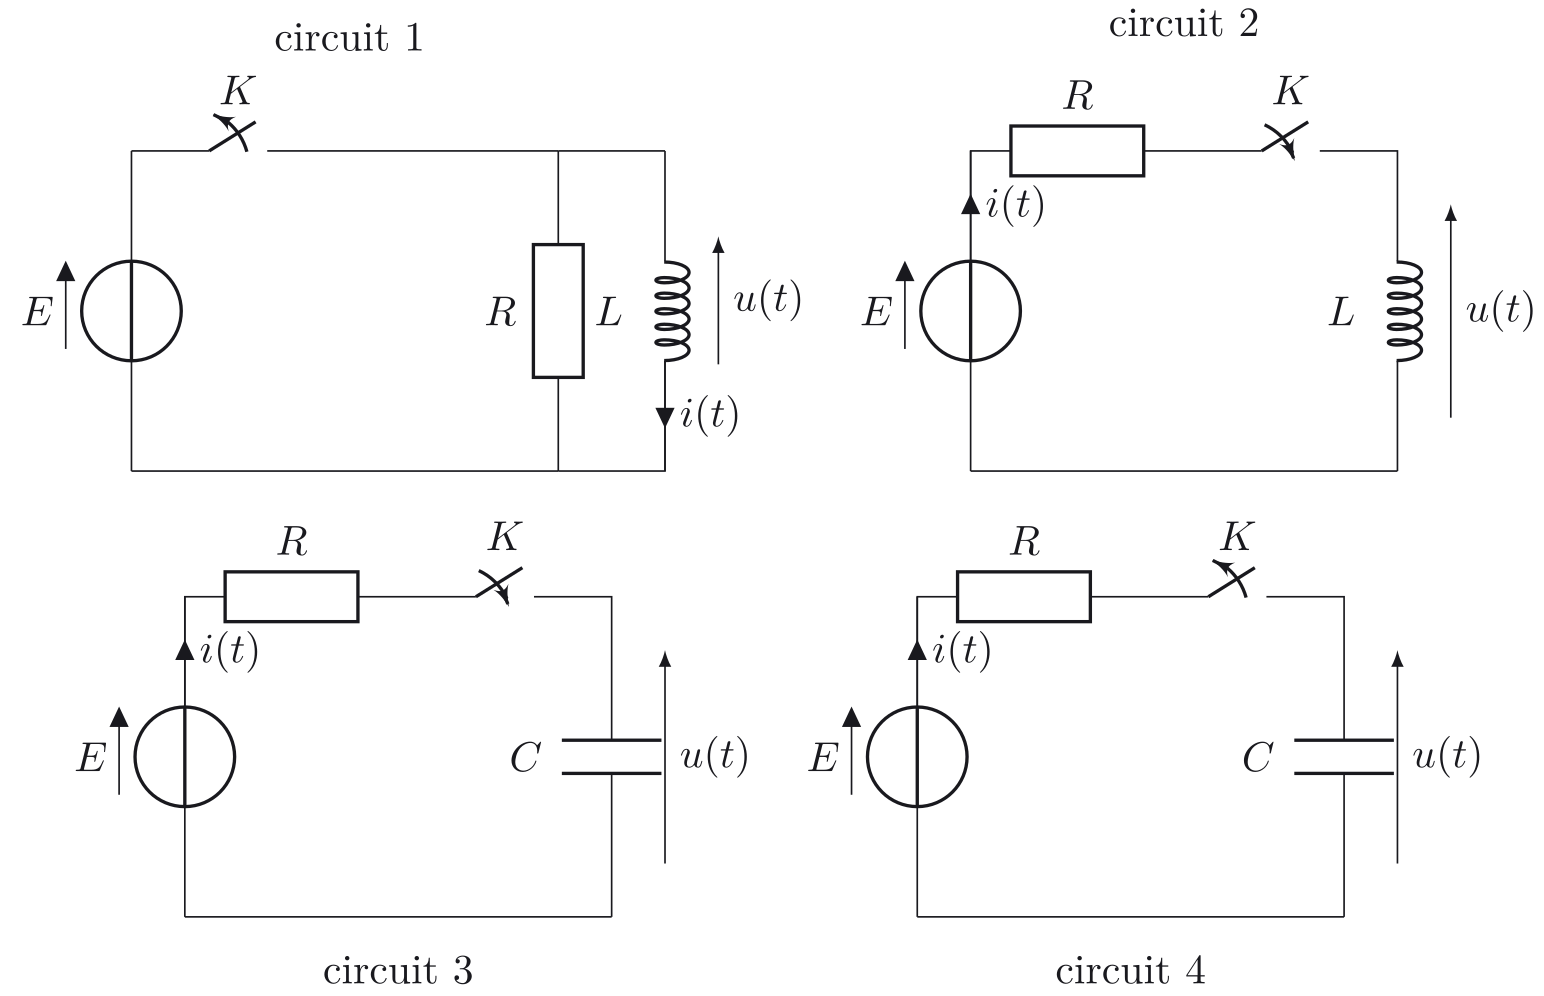
\includegraphics[width=.7\linewidth]{quelcircuit}
	\end{center}
}%

\QR{%
	Associer chaque courbe avec l'un des 4 montages ci-dessus, et calculer les
	valeurs de $E$ et $L$ ou $C$ utilisées. Tous les interrupteurs s’ouvrent ou
	se ferment à $t = 0$.
}{%
	\ifprof{%
		\vspace{-15pt}
	}%
	\begin{itemize}
		\item Pour la courbe 1~: on observe une diminution exponentielle de la
		      \textbf{tension} et une \textbf{discontinuité} de cette dernière en
		      $t=0$. Or, les condensateurs ont une tension continue à leurs
		      bornes, cette courbe ne peut donc \textbf{pas} être issue d'un
		      circuit avec un \textbf{condensateur}~: ni le 3, ni le 4.
		      \bigbreak
		      Ensuite, comme c'est forcément une bobine, on observe que $u = L
			      \dv{i}{t} > 0$, autrement dit l'intensité monte dans le circuit. Le
		      circuit 1 s'ouvre à $t=0$, donc l'intensité devrait y baisser~:
		      finalement il ne nous reste que le \textbf{circuit 2}.
		      \bigbreak
		      Dans ce circuit, la constante de temps est connue (cf.\ cours) et
		      vaut $\tau = L/R$. On la détermine avec l'intersection entre la
		      tangente en $t=0$ et l'asymptote $u=0$, où en trouvant l'instant où
		      $u$ et son asymptote ont un écart relatif de 37\%, c'est-à-dire ici
		      quand $u(\tau) = \SI{1.8}{V}$. On trouve dans tous les cas
		      \fbox{$\tau = \SI{1.0}{ms}$}, soit \fbox{$L = \SI{1.0}{H}$}.
		\item Pour la courbe 2~: on observe une augmentation exponentielle de la
		      tension et un continuité de cette dernière en $t=0$. On peut donc
		      affirmer que $u$ est la tension aux bornes d'un ondensateur, et que
		      ce dernier se charge~: on y associe donc le \textbf{circuit 3}.
		      \bigbreak
		      L'asymptote quand $t \rightarrow \infty$ est $u = E$, puisqu'alors
		      $i=0$ (comportement condensateur RP) et donc toute la tension du
		      générateur se retrouve aux bornes de $C$ (et pas de $R$ car $i=0$)~;
		      ainsi, \fbox{$E = \SI{10}{V}$}, et $u(\tau) = \SI{6.3}{V}$ ou la
		      tangente en 0 donnent \fbox{$\tau = \SI{0.070}{ms}$}~; comme ici
		      $\tau = RC$, on trouve \fbox{$C = \SI{7.0e-8}{F}$}.
	\end{itemize}
}%

\end{document}
